\documentclass[conference]{IEEEtran}
\IEEEoverridecommandlockouts

\usepackage{cite}
\usepackage{amsmath,amssymb}
\usepackage{graphicx}
\usepackage{booktabs}
\usepackage{array}
\usepackage{algorithm}
\usepackage{algpseudocode}
\usepackage{tikz}
\usetikzlibrary{arrows.meta,positioning,fit,calc}
\usepackage{pgfplots}
\pgfplotsset{compat=1.17}
\usepackage{xcolor}
\usepackage{microtype}

\algrenewcommand\algorithmicrequire{\textbf{Input:}}
\algrenewcommand\algorithmicensure{\textbf{Output:}}

\begin{document}

\title{Self-Healing Trust-Aware Predictive Maintenance: Physics-Based Fault and Attack Attribution for Industrial Pump Monitoring at the Edge}

\author{
\IEEEauthorblockN{Tejashwini A G, Durgashree R, Keerthi S and Yeshwanth L B}
\IEEEauthorblockA{Department of Computer Science and Engineering (IoT \& Cybersecurity including Blockchain)\\
B.M.S. College of Engineering, Bengaluru, India}
}

\maketitle

\begin{abstract}
A sensor that is failing and a sensor that is being falsified produce data that a conventional anomaly detector cannot tell apart, yet they demand opposite responses: maintenance for a fault, isolation for an attack. We present SHTAPM, an edge-to-dashboard monitoring system for industrial pumps that resolves this ambiguity with the physics of the machine. Motor current and vibration are treated as two independent witnesses of whether the motor is running; when their window-median states contradict each other, the anomaly is attributed as an attack on the channel that changed state alone, otherwise as a fault. Attribution is combined with an Isolation Forest detector, a Beta-reputation trust score that fuses statistical consistency, physical correlation and historical reliability, isolation of untrusted channels with LSTM digital-twin substitution bounded to 60~s, a latched safe stop, and a SHA-256 hash-chained ledger of every safety-relevant decision. The complete pipeline runs on a Raspberry~Pi~5. On a 51-minute recording of a physical pump rig with injected falsifications, the system produced no false attack attribution on 2,552 clean channel-windows, attributed 73\% of state-crossing attacks correctly while keeping 85\% of faults as faults, raising balanced accuracy from 60\% to 79\% over a trend-based baseline, and reduced the error of the served value under attack by 79--87\% out of sample. We also quantify where physical attribution ends: falsifications that keep a reading within its true physical state are indistinguishable from clean data on this rig.
\end{abstract}

\begin{IEEEkeywords}
industrial IoT, predictive maintenance, false data injection, fault--attack attribution, trust management, digital twin, edge computing
\end{IEEEkeywords}

\section{Introduction}

Pumping stations in water and wastewater networks are largely unmanned and supervised through telemetry. The same low-cost, connected sensors that enable condition-based maintenance also widen the attack surface: incidents from Stuxnet~\cite{langner2011stuxnet} to the 2021 intrusion at a water-treatment plant in Oldsmar, Florida have shown that process values can be manipulated while operators watch normal-looking data.

An anomalous reading has two very different causes. A sensor may be \emph{failing}: it drifts, spikes, freezes or stops responding. Or it may be \emph{falsified}: an attacker injects a constant, adds a bias, replays an earlier recording or ramps the value slowly~\cite{liu2009fdi,mo2009replay}. Statistical detectors flag both identically~\cite{liu2008iforest,goh2017rnn}, yet the correct responses are opposite. Recalibrating a sensor that is lying preserves the attack; isolating a healthy but noisy sensor discards information. Predictive-maintenance models, in turn, assume that their inputs are honest~\cite{lee2014phm,susto2015pdm}, so a single compromised sensor silently corrupts every downstream estimate.

This paper presents SHTAPM (Self-Healing Trust-Aware Predictive Maintenance), a complete monitoring system that runs on a single edge computer next to the pump. Its contributions are:

\begin{enumerate}
  \item \textbf{Operating-state attribution.} A model-free physics rule that uses motor current and vibration as two independent witnesses of the motor state and attributes a contradiction to the channel that changed state alone. It requires only coarse state bands learned from clean operation, not a dynamic process model.
  \item \textbf{Evidence-fusing trust with automatic response.} A Beta-reputation trust score per channel that combines consistency, physical-correlation and historical-reliability evidence, whose steady state equals the evidence level and which drives isolation and release with hysteresis.
  \item \textbf{Bounded self-healing and auditable autonomy.} Digital-twin substitution of isolated channels with an explicit time budget that ends in a latched safe stop, and a hash-chained ledger of decisions rather than raw data.
  \item \textbf{Evaluation on physical hardware.} Ground-truth injections into recordings of a physical rig, live tests on the running system, a comparison with a trend-based attribution baseline, results on the public SWaT dataset~\cite{goh2016swat}, and a quantified limit of physical attribution.
\end{enumerate}

\section{Related Work}

\textbf{Predictive maintenance.} PHM for rotating machinery maps vibration and current features to health states and remaining useful life~\cite{lee2014phm,zhao2019dlhealth}, and machine learning schedules maintenance more economically than fixed intervals~\cite{susto2015pdm}. Benchmarks such as CWRU~\cite{smith2015cwru} and PRONOSTIA~\cite{nectoux2012pronostia} contain only honest sensors, so these methods are not evaluated against falsified inputs.

\textbf{Anomaly and attack detection.} Isolation Forest~\cite{liu2008iforest} and recurrent or convolutional predictors~\cite{malhotra2015lstm,goh2017rnn,kravchik2018cnn} detect attacks on testbeds such as SWaT~\cite{goh2016swat}, and stealthy attacks within detector noise bound what any statistical detector can achieve~\cite{urbina2016stealthy}. These detectors raise an alarm; they do not explain whether its cause is a fault or an attack, and monitoring of the affected quantity stops.

\textbf{Physics- and model-based methods.} Physics-based detection checks invariants of the process~\cite{giraldo2018physics} or sensor noise fingerprints~\cite{ahmed2018noise}. Analytical redundancy~\cite{chow1984redundancy} and model-based diagnosis~\cite{isermann2005fdd} isolate faulty sensors through parity relations, and Pasqualetti \emph{et al.}~\cite{pasqualetti2013identification} characterise when attacks are detectable and identifiable. These methods require an accurate, typically linear, dynamic model, which is rarely available for a low-cost installation. We instead exploit coarse, qualitative redundancy (whether a motor runs) that is robust without such a model; the undetectable attacks predicted by~\cite{pasqualetti2013identification} reappear in our results as within-state attacks.

\textbf{Trust, twins and logging.} Beta reputation~\cite{josang2002beta} and its use in sensor networks and the IoT~\cite{ganeriwal2008reputation,bao2012dynamic} rely mostly on agreement between neighbours. Digital twins are used for monitoring and prognosis~\cite{tao2019twin}, not to stand in for a distrusted sensor under a time bound. Hash chains~\cite{haber1991timestamp} and lightweight IoT ledgers~\cite{dorri2017optimized} usually record data rather than the decisions of an autonomous system.

\section{System Overview and Threat Model}

\begin{figure}[t]
\centering
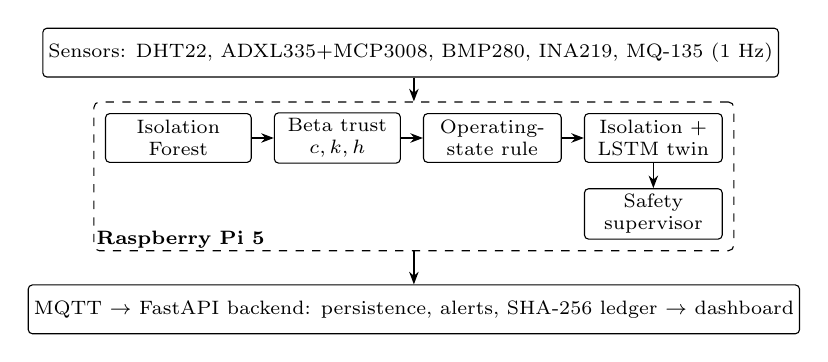
\begin{tikzpicture}[
  box/.style={draw, rounded corners=1.5pt, align=center, font=\scriptsize, minimum height=0.62cm, inner sep=2pt, fill=white},
  fl/.style={-{Stealth[length=1.6mm]}, semithick},
  node distance=0.32cm and 0.28cm]
  \node[box, minimum width=7.9cm] (s) {Sensors: DHT22, ADXL335+MCP3008, BMP280, INA219, MQ-135 (1~Hz)};
  \node[box, below=0.45cm of s, xshift=-2.95cm, minimum width=1.85cm] (d) {Isolation\\Forest};
  \node[box, right=of d, minimum width=1.6cm] (t) {Beta trust\\$c,k,h$};
  \node[box, right=of t, minimum width=1.75cm] (a) {Operating-\\state rule};
  \node[box, right=of a, minimum width=1.75cm] (h) {Isolation +\\LSTM twin};
  \node[box, below=0.32cm of h, minimum width=1.75cm] (sv) {Safety\\supervisor};
  \node[draw, dashed, rounded corners=2pt, fit=(d)(h)(sv), inner sep=4pt] (edge) {};
  \node[font=\scriptsize\bfseries, anchor=south west, inner sep=1pt] at (edge.south west) {Raspberry Pi 5};
  \node[box, below=0.42cm of edge, minimum width=7.9cm] (b) {MQTT $\rightarrow$ FastAPI backend: persistence, alerts, SHA-256 ledger $\rightarrow$ dashboard};
  \draw[fl] (s.south -| edge.north) -- (edge.north);
  \draw[fl] (d) -- (t); \draw[fl] (t) -- (a); \draw[fl] (a) -- (h); \draw[fl] (h) -- (sv);
  \draw[fl] (edge.south) -- (b.north);
\end{tikzpicture}
\caption{SHTAPM architecture. All decisions are made on the edge node; the backend observes and records.}
\label{fig:arch}
\end{figure}

Fig.~\ref{fig:arch} shows the architecture. A Raspberry Pi~5 samples six channels (temperature, humidity, vibration, pressure, motor current and gas) at 1~Hz. A window of the last $W = 30$ samples is evaluated with every new frame by the detector, the trust engine and the attribution rule; untrusted channels are isolated and substituted, and a safety supervisor is the only component allowed to switch the pump relay. Decisions and actuation are published over MQTT to a FastAPI backend that persists them, raises alerts, chains safety-relevant events into a ledger and serves a role-based dashboard. Because the decision loop runs entirely on the edge, protection does not depend on the network.

\textbf{Threat model.} The adversary can falsify the values reported by one sensor channel between the sensor and the decision pipeline, for example by spoofing, bias or ramp injection, or replay. The adversary does not control the physical process or a second, physically coupled sensor at the same time, and does not compromise the edge node itself. Physical faults (drift, spikes, stuck output, dropouts, loose connections) occur independently.

\section{Methods}

\subsection{Detection}

Each $30 \times 6$ window is flattened into a 180-dimensional point and scored by an Isolation Forest~\cite{liu2008iforest} of 100 trees fitted on windows of a clean recording of the rig. Instead of thresholding raw scores, we store the clean score distribution and report the severity of a window as the empirical CDF of its score within it, $\mathrm{sev} \in [0, 1]$, flagging windows with $\mathrm{sev} \geq 0.90$. The detector is deliberately sensitive (about 10\% of clean windows are flagged by construction); trust and attribution decide which flags matter. Flags are localised to channels with a two-sided test on each channel's window variance against its own clean distribution, which catches both spikes or constant spoofs (abnormally low normalised variance) and noisy behaviour.

\subsection{Evidence-Fusing Beta Trust}

Each channel holds a Beta state $(\alpha, \beta)$, $\alpha_0 = \beta_0 = 1$, with trust $T = \alpha / (\alpha + \beta)$. Every window supplies evidence $g \in [0, 1]$ from three independent terms. \emph{Consistency} $c = 1 - F_r(r)$, where $r$ is the RMS of the window's z-scores against the baseline mean and deviation and $F_r$ its clean empirical CDF. \emph{Physical correlation} $k \in \{0, 1\}$ is set to $0$ for the channel named as suspect by the attribution rule. \emph{Historical reliability} $h_t = \gamma h_{t-1} + (1 - \gamma) o_t$, with $\gamma = 0.95$ and $o_t = 1$ when the channel was not flagged. The update is
\begin{align}
g &= 0.4c + 0.3k + 0.3h, \\
\alpha_t &= \lambda \alpha_{t-1} + g, \quad
\beta_t = \lambda \beta_{t-1} + 1 - g,
\end{align}
with forgetting factor $\lambda = 0.7$. Under constant evidence the state converges to $\alpha^{*} = g/(1-\lambda)$, $\beta^{*} = (1-g)/(1-\lambda)$, hence
\begin{equation}
T^{*} = \alpha^{*} / (\alpha^{*} + \beta^{*}) = g,
\end{equation}
so trust is bounded, interpretable and settles at the evidence level (Fig.~\ref{fig:trust}). Channels are Trusted ($T \geq 0.7$), Suspicious ($0.4 \leq T < 0.7$) or Malicious ($T < 0.4$). Under fully adverse evidence trust falls from Trusted to Malicious within three windows, but because $h$ recovers slowly it returns to Trusted only after about 21 clean windows: a sensor that has lied must earn its trust back.

\begin{figure}[t]
\centering
\begin{tikzpicture}
\begin{axis}[
  width=\columnwidth, height=4.2cm,
  xlabel={Window index}, ylabel={Value},
  xmin=0, xmax=120, ymin=0, ymax=1.02, ytick={0,0.4,0.7,1},
  tick label style={font=\scriptsize}, label style={font=\footnotesize},
  legend style={at={(0.98,0.04)}, anchor=south east, font=\scriptsize, draw=none, fill=white, inner sep=1pt},
  grid=major, grid style={gray!20}]
\fill[gray!12] (axis cs:30,0) rectangle (axis cs:75,1.02);
\node[font=\tiny, anchor=north] at (axis cs:52,1.0) {adverse evidence};
\addplot[thick, black] table[x=t, y=trust] {data/trust.dat};
\addplot[thick, dashed, gray] table[x=t, y=evidence] {data/trust.dat};
\addplot[thin, densely dotted, black, domain=0:120] {0.7};
\addplot[thin, densely dotted, black, domain=0:120] {0.4};
\legend{trust $T$, evidence $g$}
\end{axis}
\end{tikzpicture}
\caption{Response of the trust update to idealised evidence: clean ($c{=}0.5$, $k{=}1$), 45 windows of fully adverse evidence, then clean again. Trust crosses 0.4 within three windows of the onset but regains 0.7 only 21 windows after it ends. Dotted lines: band limits.}
\label{fig:trust}
\end{figure}

\subsection{Operating-State Attribution}

A pump motor is either running or idle, and both its supply current and its vibration reflect that state. Each channel's state is estimated from the \emph{median} of its raw window, so that taps and short glitches cannot flip it:
\begin{equation}
s(\mathbf{x}) = \begin{cases}
\textsc{idle}, & \operatorname{med}(\mathbf{x}) \leq b_{\mathrm{idle}},\\
\textsc{run}, & \operatorname{med}(\mathbf{x}) \geq b_{\mathrm{run}},\\
\textsc{unclear}, & \text{otherwise}.
\end{cases}
\end{equation}
For current, $b_{\mathrm{idle}} = 0.05$~A and $b_{\mathrm{run}} = 0.3$~A. Vibration depends on mounting, so its bands are learned from steady windows of the clean recording: $b_{\mathrm{idle}}$ is 1.5 times the 99.9th percentile of idle medians and $b_{\mathrm{run}}$ lies midway between $b_{\mathrm{idle}}$ and the 5th percentile of running medians (0.142~$g$ and 0.314~$g$ on our rig). The gap between bands provides hysteresis, so motor transitions never produce a verdict. Algorithm~\ref{alg:attr} gives the rule. The key observation is that a motor that really starts or stops moves \emph{both} witnesses, whereas a falsified channel moves alone.

\begin{algorithm}[t]
\caption{Operating-state attribution for one window}
\label{alg:attr}
\small
\begin{algorithmic}[1]
\Require windows $\mathbf{x}_I$ (current), $\mathbf{x}_V$ (vibration); flags $F$; previous states $s_I^-, s_V^-$
\Ensure label and suspect channel
\State $s_I \gets s(\mathbf{x}_I)$; \ $s_V \gets s(\mathbf{x}_V)$
\If{$\{s_I, s_V\} = \{\textsc{idle}, \textsc{run}\}$}
  \If{$s_I \neq s_I^-$ \textbf{and} $s_V = s_V^-$} \State suspect $\gets$ current
  \ElsIf{$s_V \neq s_V^-$ \textbf{and} $s_I = s_I^-$} \State suspect $\gets$ vibration
  \Else \ suspect $\gets$ both
  \EndIf
  \State \Return (\textsc{attack}, suspect)
\ElsIf{any channel in $F$ is flagged}
  \State \Return (\textsc{fault}, flagged channels)
\Else \ \Return (\textsc{none})
\EndIf
\end{algorithmic}
\end{algorithm}

\subsection{Bounded Self-Healing and Safe Stop}

A channel is isolated when $T < 0.4$ and released when $T \geq 0.7$. While isolated, its value is replaced by a single-layer LSTM~\cite{hochreiter1997lstm} reconstruction (32 hidden units) whose input is the 30-sample window with the isolated channel zeroed plus a one-hot mask. The deployed twin reconstructs current from vibration; ambient channels were excluded after a leave-one-recording-out study showed that they degrade accuracy on other days (skill $-$122.7\% versus +38.5\% on the hardest held-out recording). Inputs and target use a fixed z-score scale, so outputs convert exactly to amperes.

Substitution is bounded: after 60~s of continuous substitution, the safety supervisor performs a \emph{latched} safe stop that only an administrator can clear. The supervisor also stops the pump on a watchdog timeout (10~s without a healthy frame) and on a dry-run signature, and forces the relay off at start-up, at shutdown and, through the service manager, after a crash. A divergence-based escalation (live reading versus twin) is implemented but disabled: on clean held-out data a $3\sigma$ threshold would have caused false stops in 4.5\% of windows.

\subsection{Decision Ledger}

Trust drops, isolations, releases, safe stops, relay commands and test injections are chained as
\begin{equation}
H_n = \mathrm{SHA256}\big(n \,\|\, \tau_n \,\|\, \mathrm{SHA256}(\mathrm{canon}(P_n)) \,\|\, H_{n-1}\big),
\end{equation}
with timestamp $\tau_n$ and canonical JSON payload $P_n$, so any modification of a past decision breaks every later link.

\section{Experimental Setup}

\textbf{Rig.} A 130-size brushed DC motor stands in for the pump. Current is measured by an INA219 (0.1~$\Omega$ shunt) in series with its supply and vibration by an ADXL335, read through a 10-bit MCP3008, mounted on the motor body; a DHT22 and a BMP280 provide ambient channels. The gas channel and the pump relay are implemented end to end in software (an MQ-135 driver with its signal conditioning, and a supervised relay with latching stops); in the reported experiments both were driven through configurable emulated sources, which share the data path with the physical drivers, so they carry no weight in any result below.

\begin{figure}[t]
\centering
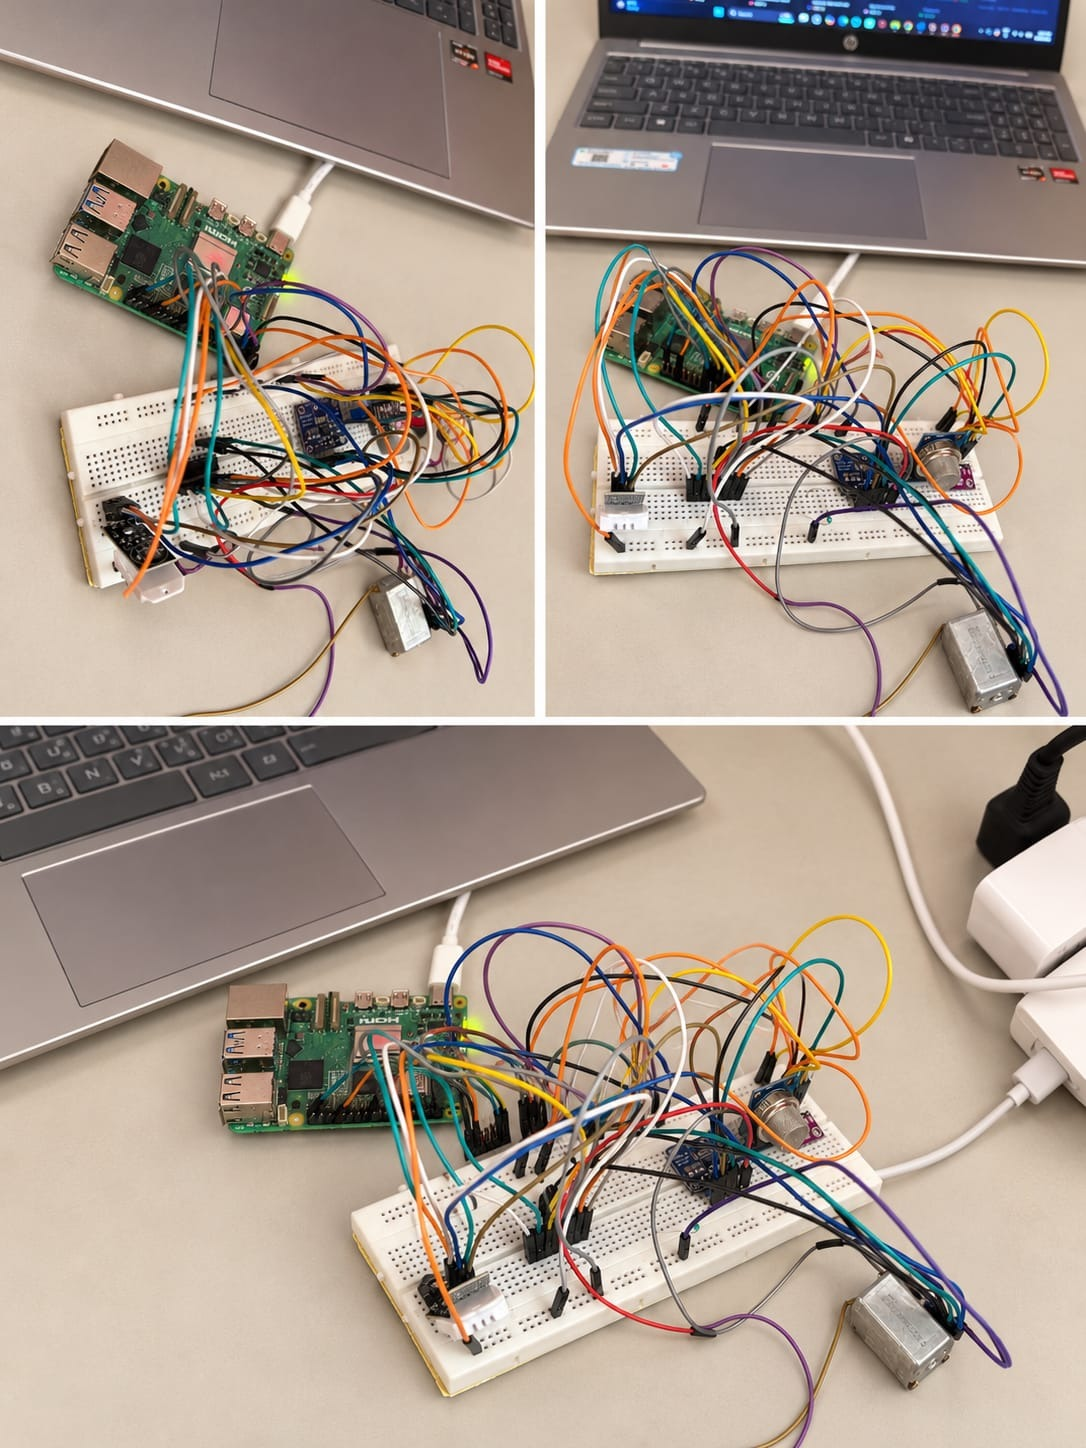
\includegraphics[width=0.62\columnwidth]{figures/bench-rig.jpg}
\caption{The bench rig: Raspberry Pi~5 edge node, sensor modules on a breadboard and the DC motor.}
\label{fig:rig}
\end{figure}

\textbf{Data.} The main dataset is a 51.4-minute clean recording (2,609 frames, no gap over 2~s) with 21 motor runs switched by hand at random intervals. Fig.~\ref{fig:medians} shows that its window medians form two separated clusters and leave the physically impossible regions empty. Earlier recordings of the rig (7.2-h idle, 19-min cycling, 25-min running) are used for robustness, and SWaT.A1~\cite{goh2016swat} for detection.

\begin{figure}[t]
\centering
\begin{tikzpicture}
\begin{axis}[
  width=\columnwidth, height=5.4cm,
  xlabel={Window median current (A)}, ylabel={Median vibration ($g$)},
  xmin=-0.05, xmax=1.0, ymin=-0.05, ymax=1.1,
  tick label style={font=\scriptsize}, label style={font=\footnotesize},
  legend style={at={(0.02,0.98)}, anchor=north west, font=\scriptsize, draw=none, fill=white, fill opacity=0.9, text opacity=1, inner sep=1pt},
  scatter/classes={idle={mark=o, black}, running={mark=triangle, black}, transition={mark=square*, gray}}]
\fill[gray!12] (axis cs:0.3,-0.05) rectangle (axis cs:1.0,0.142);
\fill[gray!12] (axis cs:-0.05,0.314) rectangle (axis cs:0.05,1.1);
\node[font=\tiny, align=center] at (axis cs:0.66,0.05) {impossible};
\addplot[scatter, only marks, mark size=1.3pt, scatter src=explicit symbolic] table[x=current, y=vibration, meta=state] {data/window_medians.dat};
\draw[densely dashed] (axis cs:0.05,-0.05) -- (axis cs:0.05,1.1);
\draw[densely dashed] (axis cs:0.3,-0.05) -- (axis cs:0.3,1.1);
\draw[densely dotted] (axis cs:-0.05,0.142) -- (axis cs:1.0,0.142);
\draw[densely dotted] (axis cs:-0.05,0.314) -- (axis cs:1.0,0.314);
\legend{idle, running, transition}
\end{axis}
\end{tikzpicture}
\caption{Current and vibration window medians of the clean recording (258 windows) with the state bands. Shaded: physically impossible states, which contain no clean window.}
\label{fig:medians}
\end{figure}

\textbf{Protocol.} Ground truth is obtained by injecting eight fault and attack types (drift, spike, stuck-at; bias, ramp, replay, constant spoof, adaptive stealth) into the recordings at random onsets, ten per scenario, and replaying them through the exact live pipeline. Attacks are grouped by measurement into those whose injected reading crosses into the opposite motor state and those that stay within the true state. An episode is scored \emph{attack} if any flagged window was attributed attack (faults are scored the same way, so false accusations count); \emph{settled} attribution is the majority label. Because labelling everything as attack would score perfectly on attacks, we report balanced accuracy $\mathrm{BA} = (\mathrm{Recall}_{\mathrm{attack}} + \mathrm{Recall}_{\mathrm{fault}})/2$. Injection magnitudes are fixed settings; no threshold was tuned on evaluation data.

\section{Results}

\subsection{False Alarms on Clean Data}

Fitted on the first 80\% of the clean recording and scored on the remaining 493 windows, the detector flagged 19.9\% of windows, as intended for a sensitive first stage, yet no channel ever entered the Malicious band and no channel was isolated. Median clean trust was 0.75--0.83 on every channel, so every isolated channel can be released once its input is clean.

\subsection{Fault and Attack Attribution}

\begin{table}[t]
\centering
\caption{Attribution on the clean recording with injections}
\label{tab:attr}
\footnotesize
\setlength{\tabcolsep}{4pt}
\begin{tabular}{@{}lcc@{}}
\toprule
Measure & Trend-sign & Operating-state \\
\midrule
State-crossing attacks, episode & 35/42 (83\%) & 32/44 (73\%) \\
State-crossing attacks, settled & 4/42 (10\%) & 29/44 (66\%) \\
Within-state attacks, episode & 12/23 (52\%) & 0/23 (0\%) \\
Faults kept as faults, episode & 10/27 (37\%) & 23/27 (85\%) \\
False attacks, clean channel-windows & 23/2552 (0.9\%) & \textbf{0/2552 (0\%)} \\
Balanced accuracy, episode & 60\% & \textbf{79\%} \\
\bottomrule
\end{tabular}
\end{table}

Table~\ref{tab:attr} compares the operating-state rule with a trend-sign baseline that labels an anomaly as attack when current and vibration trend in opposite directions within a window. The baseline's higher attack recall is not discrimination: it also labelled half of the physically consistent attacks and almost two thirds of genuine faults as attacks, and raised false attacks on clean data. The operating-state rule never accused a clean channel, kept 85\% of faults as faults and raised balanced accuracy from 60\% to 79\%. Per scenario, bias and replay across states were attributed in 10/10 and 9/10 detected episodes (settled), and spikes and stuck sensors were always kept as faults; the remaining fault errors are drifts, which share their waveform with ramp attacks. On the earlier recordings the rule attributed 120/120, 12/12 and 63/70 state-crossing attacks with at most 0.1\% false attacks on clean data.

\textbf{Real physical events.} In a guided session, taps on the accelerometer with the motor off or running, and removing its power, were all attributed as faults; the only isolation was of the accelerometer that had genuinely lost power, and two attack windows occurred at one motor switch-on.

\subsection{Self-Healing}

\begin{table}[t]
\centering
\caption{Self-healing of the current channel (12 attacks each; twin not trained on this recording)}
\label{tab:heal}
\footnotesize
\setlength{\tabcolsep}{4pt}
\begin{tabular}{@{}lcc@{}}
\toprule
Measure & Bias & Constant spoof \\
\midrule
Attacks isolated & 10/12 & 10/12 \\
Time to isolate, median & $\approx$21~s & $\approx$18~s \\
Error without healing, median & 0.60~A & 0.57~A \\
Error of served twin value, median & \textbf{0.079~A} & \textbf{0.12~A} \\
False isolations on clean data & 0 & 0 \\
\bottomrule
\end{tabular}
\end{table}

Table~\ref{tab:heal} shows that, out of sample, the twin removed 79--87\% of the error that the falsified reading would otherwise have introduced. On its own held-out data its skill against a mean predictor is +47.3\% (RMSE 0.188~A versus 0.357~A).

\subsection{Running System}

On the live system, a spoof of the current reading to 0~A while the motor ran was attributed as an attack and isolated within 21--23~s, with the twin serving 0.791~A while the sensor claimed 0~A; a +0.8~A bias with the motor off was attributed as an attack after 19~s; a stuck current sensor was reported as a fault. An attack held beyond the substitution budget produced the latched safe stop exactly 60~s after isolation, and the ledger verified intact. The complete decision cycle sustained the 1~Hz sampling rate throughout. Fig.~\ref{fig:ui} shows the control room during such an attack.

\begin{figure*}[t]
\centering
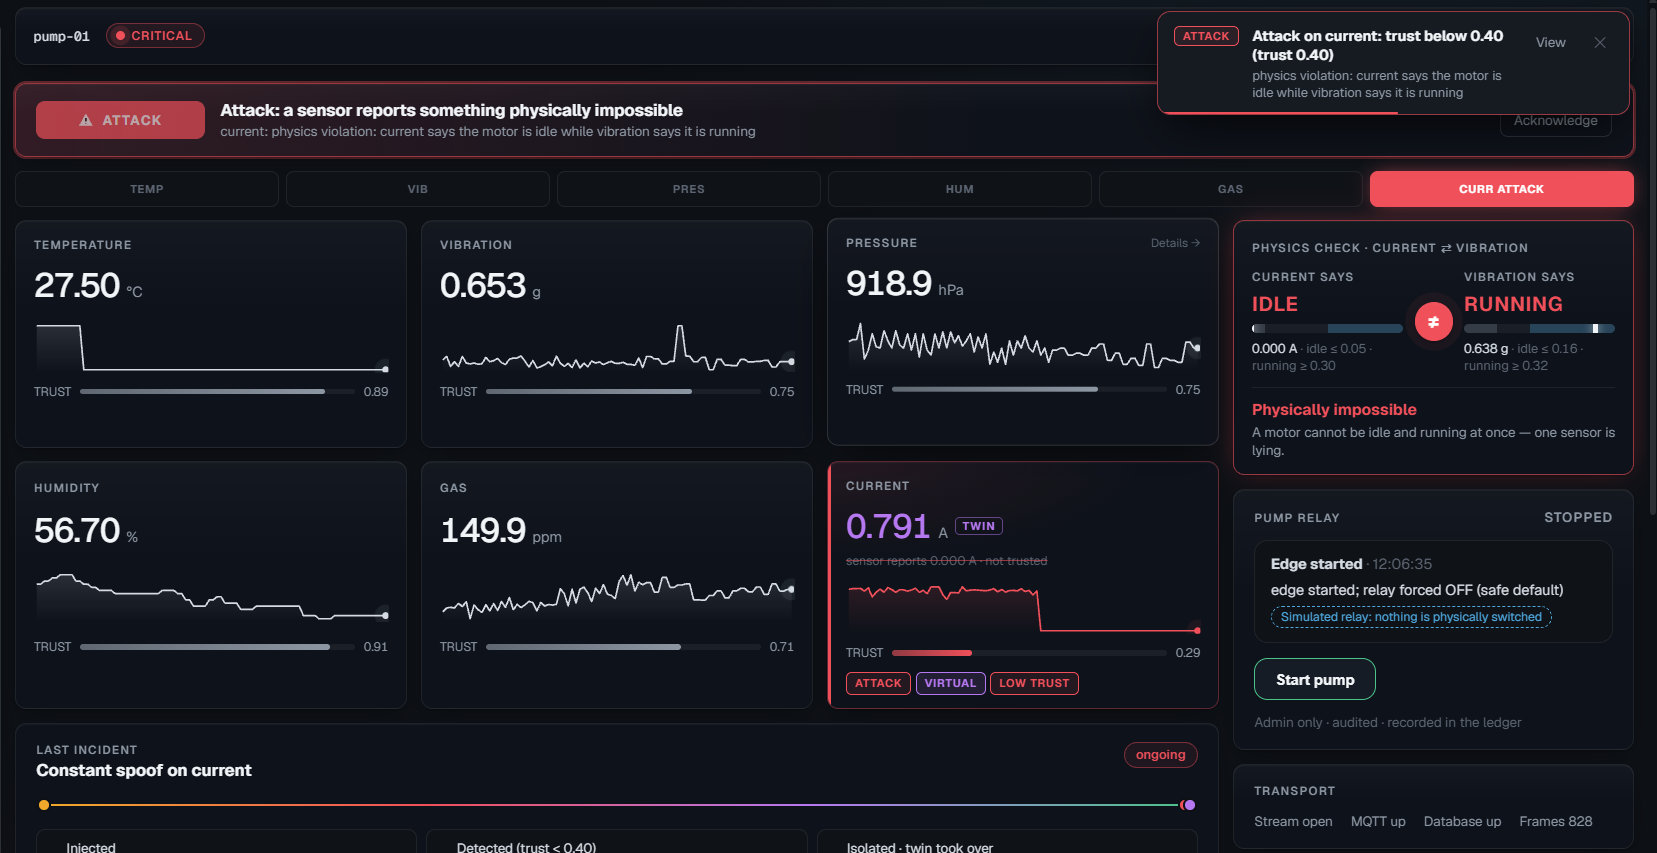
\includegraphics[width=0.82\textwidth]{figures/controlroom-attack.png}
\caption{Control room during a constant-spoof attack on the current sensor: the physics panel reports an impossible state (current idle, vibration running), the channel is attributed as an attack and isolated, and the twin's value (0.791~A) is shown in place of the sensor's 0~A.}
\label{fig:ui}
\end{figure*}

\subsection{Detection on SWaT}

\begin{table}[t]
\centering
\caption{Detection on SWaT.A1 (thresholds at each detector's nominal 5\% clean-flag rate)}
\label{tab:swat}
\footnotesize
\setlength{\tabcolsep}{3.5pt}
\begin{tabular}{@{}lcccc@{}}
\toprule
Detector & Prec. & Rec. & $F_1$ & Events/35 \\
\midrule
Isolation Forest (deployed) & 0.418 & 0.332 & 0.370 & 32 \\
Isolation Forest, low-pass & 0.548 & 0.562 & 0.555 & 33 \\
Per-channel z-score & 0.799 & 0.687 & 0.739 & 13 \\
max(z-score, IF low-pass) & 0.543 & 0.746 & 0.629 & 33 \\
\bottomrule
\end{tabular}
\end{table}

Table~\ref{tab:swat} shows that window-level $F_1$ and event coverage pull apart: the z-score detector is most precise but misses 22 of 35 attacks, whereas the Isolation Forest flags nearly every attack event. In SHTAPM this trade is deliberate, since trust and attribution remove false flags downstream; low-pass filtering improves the detector's $F_1$ from 0.370 to 0.555 at equal coverage and is a direct improvement.

\subsection{Where Physical Attribution Ends}

No within-state attack was attributed (Table~\ref{tab:attr}). To test whether the twin provides a second witness for such attacks, we computed the residual between the twin's prediction and measured running current on held-out data: its clean 99.9th percentile is 0.48~A, and an in-state bias exceeds it in fewer than 2\% of windows up to 0.4~A but in 72\% at 0.6~A, about 80\% of the running current. Small in-state falsifications are therefore physically consistent with every other sensor on this rig, as predicted by the identifiability limits of~\cite{pasqualetti2013identification}; exposing them requires evidence beyond sensor readings, such as sensor attestation or physical watermarking~\cite{mo2009replay}.

\section{Discussion and Limitations}

The operating-state rule trades some attack recall for an accusation that is never false on clean data, which we consider the property that matters to an operator: a false accusation triggers a security response against a healthy sensor. Its coverage is limited to physically coupled channels; on our bench only current and vibration are coupled, so the ambient channels can be attributed only as faults, while on a real pump discharge pressure and flow would add further witnesses. Drift and ramp are indistinguishable without additional evidence. The rig is a small DC motor rather than a pump, so dry-run protection was verified on injected frames, the gas and relay paths were exercised through emulated sources, and the bench broker was unauthenticated. Validation on a full-scale pump with a physical relay is the natural next step. Remaining-useful-life prognosis and a learned response policy are implemented as modules but not deployed, because they require run-to-failure data from the target pump and agreed reward weights, respectively.

\section{Conclusion}

SHTAPM shows that physical redundancy between two inexpensive sensors can turn ``something is anomalous'' into ``this sensor is lying'' on a low-cost edge device, without a dynamic process model. Combined with evidence-fusing trust, bounded digital-twin substitution, a latched safe stop and a decision ledger, it keeps a pump monitored and accountable while one of its sensors is falsified, produced no false attack on clean data, and states precisely where physical evidence runs out.

\begin{thebibliography}{99}
\footnotesize

\bibitem{langner2011stuxnet} R. Langner, ``Stuxnet: Dissecting a cyberwarfare weapon,'' \emph{IEEE Security \& Privacy}, vol. 9, no. 3, pp. 49--51, 2011.

\bibitem{liu2009fdi} Y. Liu, P. Ning and M. K. Reiter, ``False data injection attacks against state estimation in electric power grids,'' in \emph{Proc. ACM CCS}, 2009, pp. 21--32.

\bibitem{mo2009replay} Y. Mo and B. Sinopoli, ``Secure control against replay attacks,'' in \emph{Proc. 47th Allerton Conf. Communication, Control, and Computing}, 2009, pp. 911--918.

\bibitem{liu2008iforest} F. T. Liu, K. M. Ting and Z.-H. Zhou, ``Isolation forest,'' in \emph{Proc. IEEE ICDM}, 2008, pp. 413--422.

\bibitem{goh2017rnn} J. Goh, S. Adepu, M. Tan and Z. S. Lee, ``Anomaly detection in cyber physical systems using recurrent neural networks,'' in \emph{Proc. IEEE HASE}, 2017, pp. 140--145.

\bibitem{lee2014phm} J. Lee, F. Wu, W. Zhao, M. Ghaffari, L. Liao and D. Siegel, ``Prognostics and health management design for rotary machinery systems---Reviews, methodology and applications,'' \emph{Mech. Syst. Signal Process.}, vol. 42, no. 1--2, pp. 314--334, 2014.

\bibitem{susto2015pdm} G. A. Susto, A. Schirru, S. Pampuri, S. McLoone and A. Beghi, ``Machine learning for predictive maintenance: A multiple classifier approach,'' \emph{IEEE Trans. Ind. Informat.}, vol. 11, no. 3, pp. 812--820, 2015.

\bibitem{goh2016swat} J. Goh, S. Adepu, K. N. Junejo and A. Mathur, ``A dataset to support research in the design of secure water treatment systems,'' in \emph{Proc. CRITIS}, LNCS 10242, 2017, pp. 88--99.

\bibitem{zhao2019dlhealth} R. Zhao, R. Yan, Z. Chen, K. Mao, P. Wang and R. X. Gao, ``Deep learning and its applications to machine health monitoring,'' \emph{Mech. Syst. Signal Process.}, vol. 115, pp. 213--237, 2019.

\bibitem{smith2015cwru} W. A. Smith and R. B. Randall, ``Rolling element bearing diagnostics using the Case Western Reserve University data: A benchmark study,'' \emph{Mech. Syst. Signal Process.}, vol. 64--65, pp. 100--131, 2015.

\bibitem{nectoux2012pronostia} P. Nectoux \emph{et al.}, ``PRONOSTIA: An experimental platform for bearings accelerated degradation tests,'' in \emph{Proc. IEEE PHM}, 2012, pp. 1--8.

\bibitem{malhotra2015lstm} P. Malhotra, L. Vig, G. Shroff and P. Agarwal, ``Long short term memory networks for anomaly detection in time series,'' in \emph{Proc. ESANN}, 2015, pp. 89--94.

\bibitem{kravchik2018cnn} M. Kravchik and A. Shabtai, ``Detecting cyber attacks in industrial control systems using convolutional neural networks,'' in \emph{Proc. ACM CPS-SPC}, 2018, pp. 72--83.

\bibitem{urbina2016stealthy} D. I. Urbina \emph{et al.}, ``Limiting the impact of stealthy attacks on industrial control systems,'' in \emph{Proc. ACM CCS}, 2016, pp. 1092--1105.

\bibitem{giraldo2018physics} J. Giraldo \emph{et al.}, ``A survey of physics-based attack detection in cyber-physical systems,'' \emph{ACM Comput. Surv.}, vol. 51, no. 4, pp. 76:1--76:36, 2018.

\bibitem{ahmed2018noise} C. M. Ahmed, J. Zhou and A. P. Mathur, ``Noise matters: Using sensor and process noise fingerprint to detect stealthy cyber attacks and authenticate sensors in CPS,'' in \emph{Proc. ACSAC}, 2018, pp. 566--581.

\bibitem{chow1984redundancy} E. Y. Chow and A. S. Willsky, ``Analytical redundancy and the design of robust failure detection systems,'' \emph{IEEE Trans. Autom. Control}, vol. 29, no. 7, pp. 603--614, 1984.

\bibitem{isermann2005fdd} R. Isermann, ``Model-based fault-detection and diagnosis---Status and applications,'' \emph{Annu. Rev. Control}, vol. 29, no. 1, pp. 71--85, 2005.

\bibitem{pasqualetti2013identification} F. Pasqualetti, F. D\"orfler and F. Bullo, ``Attack detection and identification in cyber-physical systems,'' \emph{IEEE Trans. Autom. Control}, vol. 58, no. 11, pp. 2715--2729, 2013.

\bibitem{josang2002beta} A. J{\o}sang and R. Ismail, ``The beta reputation system,'' in \emph{Proc. 15th Bled Electronic Commerce Conf.}, 2002, pp. 2502--2511.

\bibitem{ganeriwal2008reputation} S. Ganeriwal, L. K. Balzano and M. B. Srivastava, ``Reputation-based framework for high integrity sensor networks,'' \emph{ACM Trans. Sensor Netw.}, vol. 4, no. 3, pp. 15:1--15:37, 2008.

\bibitem{bao2012dynamic} F. Bao and I.-R. Chen, ``Dynamic trust management for Internet of Things applications,'' in \emph{Proc. Int. Workshop on Self-Aware Internet of Things}, 2012, pp. 1--6.

\bibitem{tao2019twin} F. Tao, H. Zhang, A. Liu and A. Y. C. Nee, ``Digital twin in industry: State-of-the-art,'' \emph{IEEE Trans. Ind. Informat.}, vol. 15, no. 4, pp. 2405--2415, 2019.

\bibitem{haber1991timestamp} S. Haber and W. S. Stornetta, ``How to time-stamp a digital document,'' \emph{J. Cryptology}, vol. 3, no. 2, pp. 99--111, 1991.

\bibitem{dorri2017optimized} A. Dorri, S. S. Kanhere and R. Jurdak, ``Towards an optimized blockchain for IoT,'' in \emph{Proc. IEEE/ACM IoTDI}, 2017, pp. 173--178.

\bibitem{hochreiter1997lstm} S. Hochreiter and J. Schmidhuber, ``Long short-term memory,'' \emph{Neural Comput.}, vol. 9, no. 8, pp. 1735--1780, 1997.

\end{thebibliography}

\end{document}
